\documentclass[]{article}
\usepackage{lmodern}
\usepackage{amssymb,amsmath}
\usepackage{ifxetex,ifluatex}
\usepackage{fixltx2e} % provides \textsubscript
\ifnum 0\ifxetex 1\fi\ifluatex 1\fi=0 % if pdftex
  \usepackage[T1]{fontenc}
  \usepackage[utf8]{inputenc}
\else % if luatex or xelatex
  \ifxetex
    \usepackage{mathspec}
  \else
    \usepackage{fontspec}
  \fi
  \defaultfontfeatures{Ligatures=TeX,Scale=MatchLowercase}
\fi
% use upquote if available, for straight quotes in verbatim environments
\IfFileExists{upquote.sty}{\usepackage{upquote}}{}
% use microtype if available
\IfFileExists{microtype.sty}{%
\usepackage{microtype}
\UseMicrotypeSet[protrusion]{basicmath} % disable protrusion for tt fonts
}{}
\usepackage[margin=1in]{geometry}
\usepackage{hyperref}
\hypersetup{unicode=true,
            pdftitle={CLass 5 Graphing and Plotting in R},
            pdfauthor={Luke Wang},
            pdfborder={0 0 0},
            breaklinks=true}
\urlstyle{same}  % don't use monospace font for urls
\usepackage{color}
\usepackage{fancyvrb}
\newcommand{\VerbBar}{|}
\newcommand{\VERB}{\Verb[commandchars=\\\{\}]}
\DefineVerbatimEnvironment{Highlighting}{Verbatim}{commandchars=\\\{\}}
% Add ',fontsize=\small' for more characters per line
\usepackage{framed}
\definecolor{shadecolor}{RGB}{248,248,248}
\newenvironment{Shaded}{\begin{snugshade}}{\end{snugshade}}
\newcommand{\KeywordTok}[1]{\textcolor[rgb]{0.13,0.29,0.53}{\textbf{#1}}}
\newcommand{\DataTypeTok}[1]{\textcolor[rgb]{0.13,0.29,0.53}{#1}}
\newcommand{\DecValTok}[1]{\textcolor[rgb]{0.00,0.00,0.81}{#1}}
\newcommand{\BaseNTok}[1]{\textcolor[rgb]{0.00,0.00,0.81}{#1}}
\newcommand{\FloatTok}[1]{\textcolor[rgb]{0.00,0.00,0.81}{#1}}
\newcommand{\ConstantTok}[1]{\textcolor[rgb]{0.00,0.00,0.00}{#1}}
\newcommand{\CharTok}[1]{\textcolor[rgb]{0.31,0.60,0.02}{#1}}
\newcommand{\SpecialCharTok}[1]{\textcolor[rgb]{0.00,0.00,0.00}{#1}}
\newcommand{\StringTok}[1]{\textcolor[rgb]{0.31,0.60,0.02}{#1}}
\newcommand{\VerbatimStringTok}[1]{\textcolor[rgb]{0.31,0.60,0.02}{#1}}
\newcommand{\SpecialStringTok}[1]{\textcolor[rgb]{0.31,0.60,0.02}{#1}}
\newcommand{\ImportTok}[1]{#1}
\newcommand{\CommentTok}[1]{\textcolor[rgb]{0.56,0.35,0.01}{\textit{#1}}}
\newcommand{\DocumentationTok}[1]{\textcolor[rgb]{0.56,0.35,0.01}{\textbf{\textit{#1}}}}
\newcommand{\AnnotationTok}[1]{\textcolor[rgb]{0.56,0.35,0.01}{\textbf{\textit{#1}}}}
\newcommand{\CommentVarTok}[1]{\textcolor[rgb]{0.56,0.35,0.01}{\textbf{\textit{#1}}}}
\newcommand{\OtherTok}[1]{\textcolor[rgb]{0.56,0.35,0.01}{#1}}
\newcommand{\FunctionTok}[1]{\textcolor[rgb]{0.00,0.00,0.00}{#1}}
\newcommand{\VariableTok}[1]{\textcolor[rgb]{0.00,0.00,0.00}{#1}}
\newcommand{\ControlFlowTok}[1]{\textcolor[rgb]{0.13,0.29,0.53}{\textbf{#1}}}
\newcommand{\OperatorTok}[1]{\textcolor[rgb]{0.81,0.36,0.00}{\textbf{#1}}}
\newcommand{\BuiltInTok}[1]{#1}
\newcommand{\ExtensionTok}[1]{#1}
\newcommand{\PreprocessorTok}[1]{\textcolor[rgb]{0.56,0.35,0.01}{\textit{#1}}}
\newcommand{\AttributeTok}[1]{\textcolor[rgb]{0.77,0.63,0.00}{#1}}
\newcommand{\RegionMarkerTok}[1]{#1}
\newcommand{\InformationTok}[1]{\textcolor[rgb]{0.56,0.35,0.01}{\textbf{\textit{#1}}}}
\newcommand{\WarningTok}[1]{\textcolor[rgb]{0.56,0.35,0.01}{\textbf{\textit{#1}}}}
\newcommand{\AlertTok}[1]{\textcolor[rgb]{0.94,0.16,0.16}{#1}}
\newcommand{\ErrorTok}[1]{\textcolor[rgb]{0.64,0.00,0.00}{\textbf{#1}}}
\newcommand{\NormalTok}[1]{#1}
\usepackage{graphicx,grffile}
\makeatletter
\def\maxwidth{\ifdim\Gin@nat@width>\linewidth\linewidth\else\Gin@nat@width\fi}
\def\maxheight{\ifdim\Gin@nat@height>\textheight\textheight\else\Gin@nat@height\fi}
\makeatother
% Scale images if necessary, so that they will not overflow the page
% margins by default, and it is still possible to overwrite the defaults
% using explicit options in \includegraphics[width, height, ...]{}
\setkeys{Gin}{width=\maxwidth,height=\maxheight,keepaspectratio}
\IfFileExists{parskip.sty}{%
\usepackage{parskip}
}{% else
\setlength{\parindent}{0pt}
\setlength{\parskip}{6pt plus 2pt minus 1pt}
}
\setlength{\emergencystretch}{3em}  % prevent overfull lines
\providecommand{\tightlist}{%
  \setlength{\itemsep}{0pt}\setlength{\parskip}{0pt}}
\setcounter{secnumdepth}{0}
% Redefines (sub)paragraphs to behave more like sections
\ifx\paragraph\undefined\else
\let\oldparagraph\paragraph
\renewcommand{\paragraph}[1]{\oldparagraph{#1}\mbox{}}
\fi
\ifx\subparagraph\undefined\else
\let\oldsubparagraph\subparagraph
\renewcommand{\subparagraph}[1]{\oldsubparagraph{#1}\mbox{}}
\fi

%%% Use protect on footnotes to avoid problems with footnotes in titles
\let\rmarkdownfootnote\footnote%
\def\footnote{\protect\rmarkdownfootnote}

%%% Change title format to be more compact
\usepackage{titling}

% Create subtitle command for use in maketitle
\newcommand{\subtitle}[1]{
  \posttitle{
    \begin{center}\large#1\end{center}
    }
}

\setlength{\droptitle}{-2em}

  \title{CLass 5 Graphing and Plotting in R}
    \pretitle{\vspace{\droptitle}\centering\huge}
  \posttitle{\par}
    \author{Luke Wang}
    \preauthor{\centering\large\emph}
  \postauthor{\par}
      \predate{\centering\large\emph}
  \postdate{\par}
    \date{Jan 25, 2019}


\begin{document}
\maketitle

Class 05 Graphics and plots with R

\begin{Shaded}
\begin{Highlighting}[]
\CommentTok{# Section 2A Line Plot}

\CommentTok{# Read table with header}
\NormalTok{weight <-}\StringTok{ }\KeywordTok{read.table}\NormalTok{(}\StringTok{"lecture-5-bggn213-rstats/weight_chart.txt"}\NormalTok{, }\DataTypeTok{header =} \OtherTok{TRUE}\NormalTok{)}

\NormalTok{## Line plot weight table}
\CommentTok{# type = change the type of plots plotted}
\CommentTok{# pch = change shape of points (integer value), you can use 1:15 to cycle through different }
\CommentTok{# col = color of the point, pass it through vector to alternate color  c("",""...)}
\CommentTok{# cex = how much text and symbols should be magnified}
\CommentTok{# lwd = line width}
\CommentTok{# ylim = limits for hte y axis, use vector to bound it}
\CommentTok{# xlab/ylab = name of x/y lable, in ""}

\KeywordTok{plot}\NormalTok{( weight,}\DataTypeTok{pch=}\DecValTok{15}\NormalTok{,}\DataTypeTok{type =}\StringTok{"o"}\NormalTok{, }\DataTypeTok{cex=} \FloatTok{1.5}\NormalTok{, }\DataTypeTok{lwd=}\DecValTok{2}\NormalTok{, }\DataTypeTok{ylim=}\KeywordTok{c}\NormalTok{(}\DecValTok{2}\NormalTok{,}\DecValTok{10}\NormalTok{), }\DataTypeTok{xlab=}\StringTok{"Age (months) "}\NormalTok{, }\DataTypeTok{ylab=}\StringTok{"Weight (kg)"}\NormalTok{, }\DataTypeTok{main =} \StringTok{"Baby Weight for First 9 Months"}\NormalTok{)}
\end{Highlighting}
\end{Shaded}

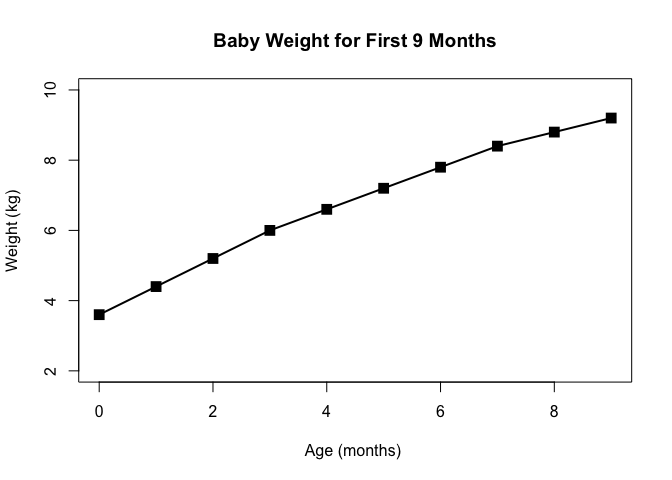
\includegraphics{class05_files/figure-latex/unnamed-chunk-1-1.pdf}

\begin{Shaded}
\begin{Highlighting}[]
\NormalTok{## Barplot of genomic features}

\CommentTok{# Read features data}
\CommentTok{# sep = \textbackslash{}t (tab)}
\NormalTok{features <-}\StringTok{ }\KeywordTok{read.table}\NormalTok{(}\StringTok{"lecture-5-bggn213-rstats/feature_counts.txt"}\NormalTok{, }\DataTypeTok{header=} \OtherTok{TRUE}\NormalTok{, }\DataTypeTok{sep =} \StringTok{"}\CharTok{\textbackslash{}t}\StringTok{"}\NormalTok{)}

\CommentTok{# Barplot}
\CommentTok{# must be vector, so specify the column with numerical values}
\CommentTok{# horiz = TRUE will set the bar plot to horizontal}
\CommentTok{# names.org = will set names of the y axis}
\CommentTok{# las, a setting in par, 1= alway horizonal, 3= always vertical}
\CommentTok{# par(mar=c()) = c(bottom, left, top, right), should be set prior to the graphic being drawn}
\CommentTok{# to resotre par, one would set the original par value to a vector then restor par value with the old par vector}
\CommentTok{# par()$mar will display the default margin}
\KeywordTok{par}\NormalTok{(}\DataTypeTok{mar=}\KeywordTok{c}\NormalTok{(}\FloatTok{5.1}\NormalTok{, }\DecValTok{7}\NormalTok{, }\FloatTok{4.1}\NormalTok{, }\FloatTok{2.1}\NormalTok{))}
\KeywordTok{barplot}\NormalTok{(features}\OperatorTok{$}\NormalTok{Count, }\DataTypeTok{horiz =} \OtherTok{TRUE}\NormalTok{, }\DataTypeTok{xlab =} \StringTok{"Counts"}\NormalTok{, }\DataTypeTok{names.arg =}\NormalTok{ features}\OperatorTok{$}\NormalTok{Feature, }\DataTypeTok{las =} \DecValTok{1}\NormalTok{, }\DataTypeTok{main =}\StringTok{"Number of Features in the Mouse GRCm38 Genome"}\NormalTok{, }\DataTypeTok{xlim =} \KeywordTok{c}\NormalTok{(}\DecValTok{0}\NormalTok{,}\DecValTok{80000}\NormalTok{))}
\end{Highlighting}
\end{Shaded}

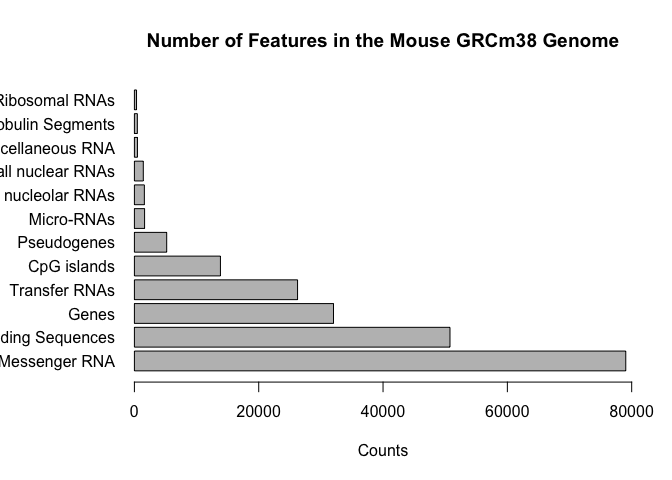
\includegraphics{class05_files/figure-latex/unnamed-chunk-1-2.pdf}

\begin{Shaded}
\begin{Highlighting}[]
\NormalTok{## Using colors in plots}
\CommentTok{# rainbow()}
\CommentTok{# heat.colors()}
\CommentTok{# cm.colors()}
\CommentTok{# topo.colors}
\CommentTok{# terrain.colors}
\NormalTok{sex_counts <-}\StringTok{ }\KeywordTok{read.table}\NormalTok{(}\StringTok{"lecture-5-bggn213-rstats/male_female_counts.txt"}\NormalTok{, }\DataTypeTok{header =} \OtherTok{TRUE}\NormalTok{, }\DataTypeTok{sep =} \StringTok{"}\CharTok{\textbackslash{}t}\StringTok{"}\NormalTok{)}

\CommentTok{# color with rainbow()}
\KeywordTok{barplot}\NormalTok{(sex_counts}\OperatorTok{$}\NormalTok{Count, }\DataTypeTok{col =} \KeywordTok{rainbow}\NormalTok{(}\KeywordTok{nrow}\NormalTok{(sex_counts)))}
\end{Highlighting}
\end{Shaded}

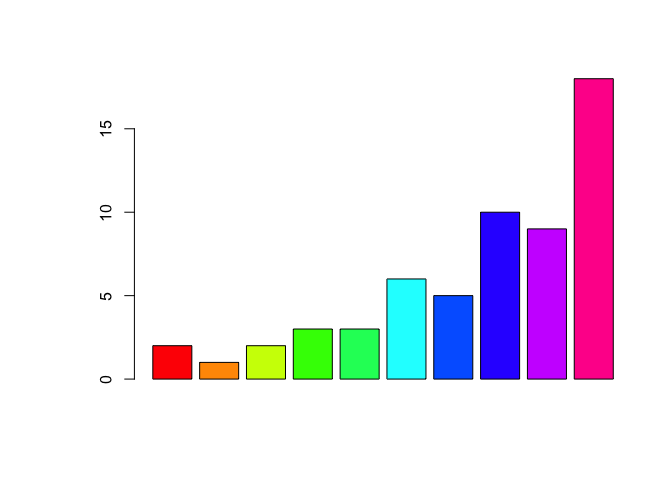
\includegraphics{class05_files/figure-latex/unnamed-chunk-1-3.pdf}

\begin{Shaded}
\begin{Highlighting}[]
\CommentTok{# color with alternating color}
\KeywordTok{barplot}\NormalTok{(sex_counts}\OperatorTok{$}\NormalTok{Count, }\DataTypeTok{col =} \KeywordTok{c}\NormalTok{(}\StringTok{"yellow"}\NormalTok{,}\StringTok{"blue"}\NormalTok{))}
\end{Highlighting}
\end{Shaded}

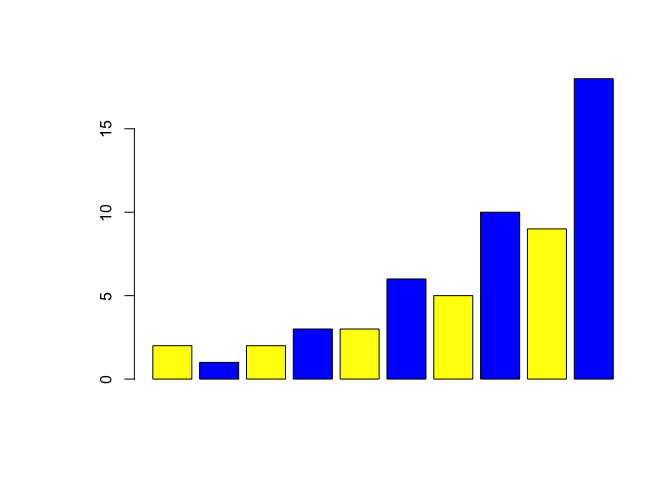
\includegraphics{class05_files/figure-latex/unnamed-chunk-1-4.pdf}

\begin{Shaded}
\begin{Highlighting}[]
\NormalTok{## Coloring by value}
\NormalTok{genes <-}\StringTok{ }\KeywordTok{read.table}\NormalTok{(}\StringTok{"lecture-5-bggn213-rstats/up_down_expression.txt"}\NormalTok{, }\DataTypeTok{header =} \OtherTok{TRUE}\NormalTok{)}

\NormalTok{state <-}\StringTok{ }\NormalTok{genes}\OperatorTok{$}\NormalTok{State }

\CommentTok{# Plot condition 1 vs. condition 2 on dot plot}
\CommentTok{# Set 3 colors using palette() to assign colors }

\KeywordTok{palette}\NormalTok{(}\KeywordTok{c}\NormalTok{(}\StringTok{"blue"}\NormalTok{,}\StringTok{"grey"}\NormalTok{, }\StringTok{"red"}\NormalTok{))}
\KeywordTok{plot}\NormalTok{(genes}\OperatorTok{$}\NormalTok{Condition1,genes}\OperatorTok{$}\NormalTok{Condition2, }\DataTypeTok{col=}\NormalTok{ state, }\DataTypeTok{ylab =} \StringTok{"Expression Condition 2"}\NormalTok{, }\DataTypeTok{xlab=}\StringTok{"Expression Condition 1"}\NormalTok{)}
\end{Highlighting}
\end{Shaded}

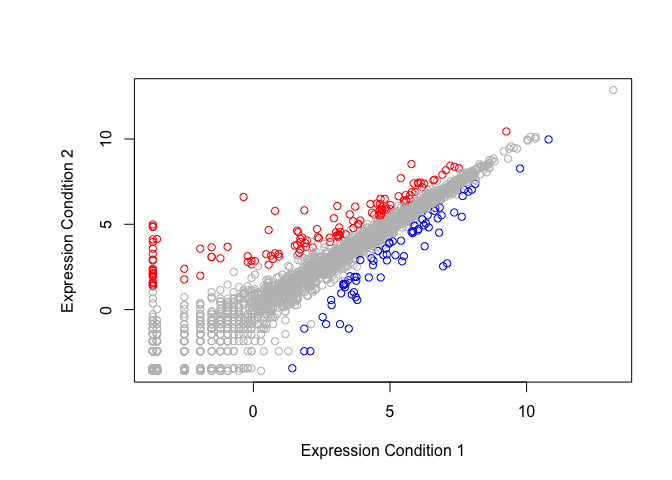
\includegraphics{class05_files/figure-latex/unnamed-chunk-1-5.pdf}

\begin{Shaded}
\begin{Highlighting}[]
\NormalTok{## Dynamic use of color, coloring by Point Density}

\NormalTok{meth <-}\StringTok{ }\KeywordTok{read.delim}\NormalTok{(}\StringTok{"lecture-5-bggn213-rstats/expression_methylation.txt"}\NormalTok{)}

\CommentTok{# densCols creates a vector of color values assigned to each point}
\NormalTok{densColors <-}\StringTok{ }\KeywordTok{densCols}\NormalTok{(meth}\OperatorTok{$}\NormalTok{gene.meth, meth}\OperatorTok{$}\NormalTok{expression)}
\KeywordTok{plot}\NormalTok{(meth}\OperatorTok{$}\NormalTok{gene.meth,meth}\OperatorTok{$}\NormalTok{expression, }\DataTypeTok{col=}\NormalTok{ densColors, }\DataTypeTok{pch=}\DecValTok{20}\NormalTok{)}
\end{Highlighting}
\end{Shaded}

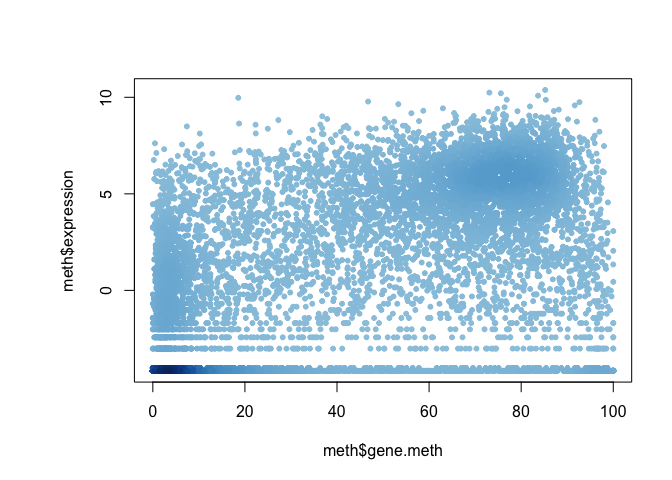
\includegraphics{class05_files/figure-latex/unnamed-chunk-1-6.pdf}

\begin{Shaded}
\begin{Highlighting}[]
\CommentTok{# Plot genes with greater than zero expression}
\CommentTok{# Using colorspaces to assign diverging HCL palette with n=3 to the plot}
\CommentTok{# Load library(colorspace)}
\KeywordTok{library}\NormalTok{(colorspace)}
\NormalTok{expressionind <-}\StringTok{ }\NormalTok{meth}\OperatorTok{$}\NormalTok{expression }\OperatorTok{>}\StringTok{ }\DecValTok{0}
\NormalTok{densColors <-}\StringTok{ }\KeywordTok{densCols}\NormalTok{(meth}\OperatorTok{$}\NormalTok{gene.meth[expressionind], meth}\OperatorTok{$}\NormalTok{expression[expressionind], }\DataTypeTok{colramp =} \KeywordTok{colorRampPalette}\NormalTok{(}\KeywordTok{diverge_hcl}\NormalTok{(}\DecValTok{3}\NormalTok{)))}
\KeywordTok{plot}\NormalTok{(meth}\OperatorTok{$}\NormalTok{gene.meth[expressionind],meth}\OperatorTok{$}\NormalTok{expression[expressionind], }\DataTypeTok{col=}\NormalTok{ densColors, }\DataTypeTok{pch=}\DecValTok{20}\NormalTok{)}
\end{Highlighting}
\end{Shaded}

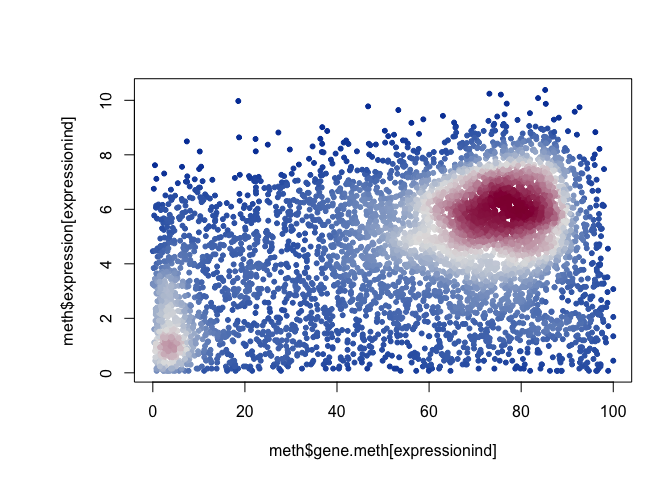
\includegraphics{class05_files/figure-latex/unnamed-chunk-1-7.pdf}


\end{document}
